\documentclass[1p]{elsarticle_modified}
%\bibliographystyle{elsarticle-num}

%\usepackage[colorlinks]{hyperref}
%\usepackage{abbrmath_seonhwa} %\Abb, \Ascr, \Acal ,\Abf, \Afrak
\usepackage{amsfonts}
\usepackage{amssymb}
\usepackage{amsmath}
\usepackage{amsthm}
\usepackage{scalefnt}
\usepackage{amsbsy}
\usepackage{kotex}
\usepackage{caption}
\usepackage{subfig}
\usepackage{color}
\usepackage{graphicx}
\usepackage{xcolor} %% white, black, red, green, blue, cyan, magenta, yellow
\usepackage{float}
\usepackage{setspace}
\usepackage{hyperref}

\usepackage{tikz}
\usetikzlibrary{arrows}

\usepackage{multirow}
\usepackage{array} % fixed length table
\usepackage{hhline}

%%%%%%%%%%%%%%%%%%%%%
\makeatletter
\renewcommand*\env@matrix[1][\arraystretch]{%
	\edef\arraystretch{#1}%
	\hskip -\arraycolsep
	\let\@ifnextchar\new@ifnextchar
	\array{*\c@MaxMatrixCols c}}
\makeatother %https://tex.stackexchange.com/questions/14071/how-can-i-increase-the-line-spacing-in-a-matrix
%%%%%%%%%%%%%%%

\usepackage[normalem]{ulem}

\newcommand{\msout}[1]{\ifmmode\text{\sout{\ensuremath{#1}}}\else\sout{#1}\fi}
%SOURCE: \msout is \stkout macro in https://tex.stackexchange.com/questions/20609/strikeout-in-math-mode

\newcommand{\cancel}[1]{
	\ifmmode
	{\color{red}\msout{#1}}
	\else
	{\color{red}\sout{#1}}
	\fi
}

\newcommand{\add}[1]{
	{\color{blue}\uwave{#1}}
}

\newcommand{\replace}[2]{
	\ifmmode
	{\color{red}\msout{#1}}{\color{blue}\uwave{#2}}
	\else
	{\color{red}\sout{#1}}{\color{blue}\uwave{#2}}
	\fi
}

\newcommand{\Sol}{\mathcal{S}} %segment
\newcommand{\D}{D} %diagram
\newcommand{\A}{\mathcal{A}} %arc


%%%%%%%%%%%%%%%%%%%%%%%%%%%%%5 test

\def\sl{\operatorname{\textup{SL}}(2,\Cbb)}
\def\psl{\operatorname{\textup{PSL}}(2,\Cbb)}
\def\quan{\mkern 1mu \triangleright \mkern 1mu}

\theoremstyle{definition}
\newtheorem{thm}{Theorem}[section]
\newtheorem{prop}[thm]{Proposition}
\newtheorem{lem}[thm]{Lemma}
\newtheorem{ques}[thm]{Question}
\newtheorem{cor}[thm]{Corollary}
\newtheorem{defn}[thm]{Definition}
\newtheorem{exam}[thm]{Example}
\newtheorem{rmk}[thm]{Remark}
\newtheorem{alg}[thm]{Algorithm}

\newcommand{\I}{\sqrt{-1}}
\begin{document}

%\begin{frontmatter}
%
%\title{Boundary parabolic representations of knots up to 8 crossings}
%
%%% Group authors per affiliation:
%\author{Yunhi Cho} 
%\address{Department of Mathematics, University of Seoul, Seoul, Korea}
%\ead{yhcho@uos.ac.kr}
%
%
%\author{Seonhwa Kim} %\fnref{s_kim}}
%\address{Center for Geometry and Physics, Institute for Basic Science, Pohang, 37673, Korea}
%\ead{ryeona17@ibs.re.kr}
%
%\author{Hyuk Kim}
%\address{Department of Mathematical Sciences, Seoul National University, Seoul 08826, Korea}
%\ead{hyukkim@snu.ac.kr}
%
%\author{Seokbeom Yoon}
%\address{Department of Mathematical Sciences, Seoul National University, Seoul, 08826,  Korea}
%\ead{sbyoon15@snu.ac.kr}
%
%\begin{abstract}
%We find all boundary parabolic representation of knots up to 8 crossings.
%
%\end{abstract}
%\begin{keyword}
%    \MSC[2010] 57M25 
%\end{keyword}
%
%\end{frontmatter}

%\linenumbers
%\tableofcontents
%
\newcommand\colored[1]{\textcolor{white}{\rule[-0.35ex]{0.8em}{1.4ex}}\kern-0.8em\color{red} #1}%
%\newcommand\colored[1]{\textcolor{white}{ #1}\kern-2.17ex	\textcolor{white}{ #1}\kern-1.81ex	\textcolor{white}{ #1}\kern-2.15ex\color{red}#1	}

{\Large $\underline{12a_{0706}~(K12a_{0706})}$}

\setlength{\tabcolsep}{10pt}
\renewcommand{\arraystretch}{1.6}
\vspace{1cm}\begin{tabular}{m{100pt}>{\centering\arraybackslash}m{274pt}}
\multirow{5}{120pt}{
	\centering
	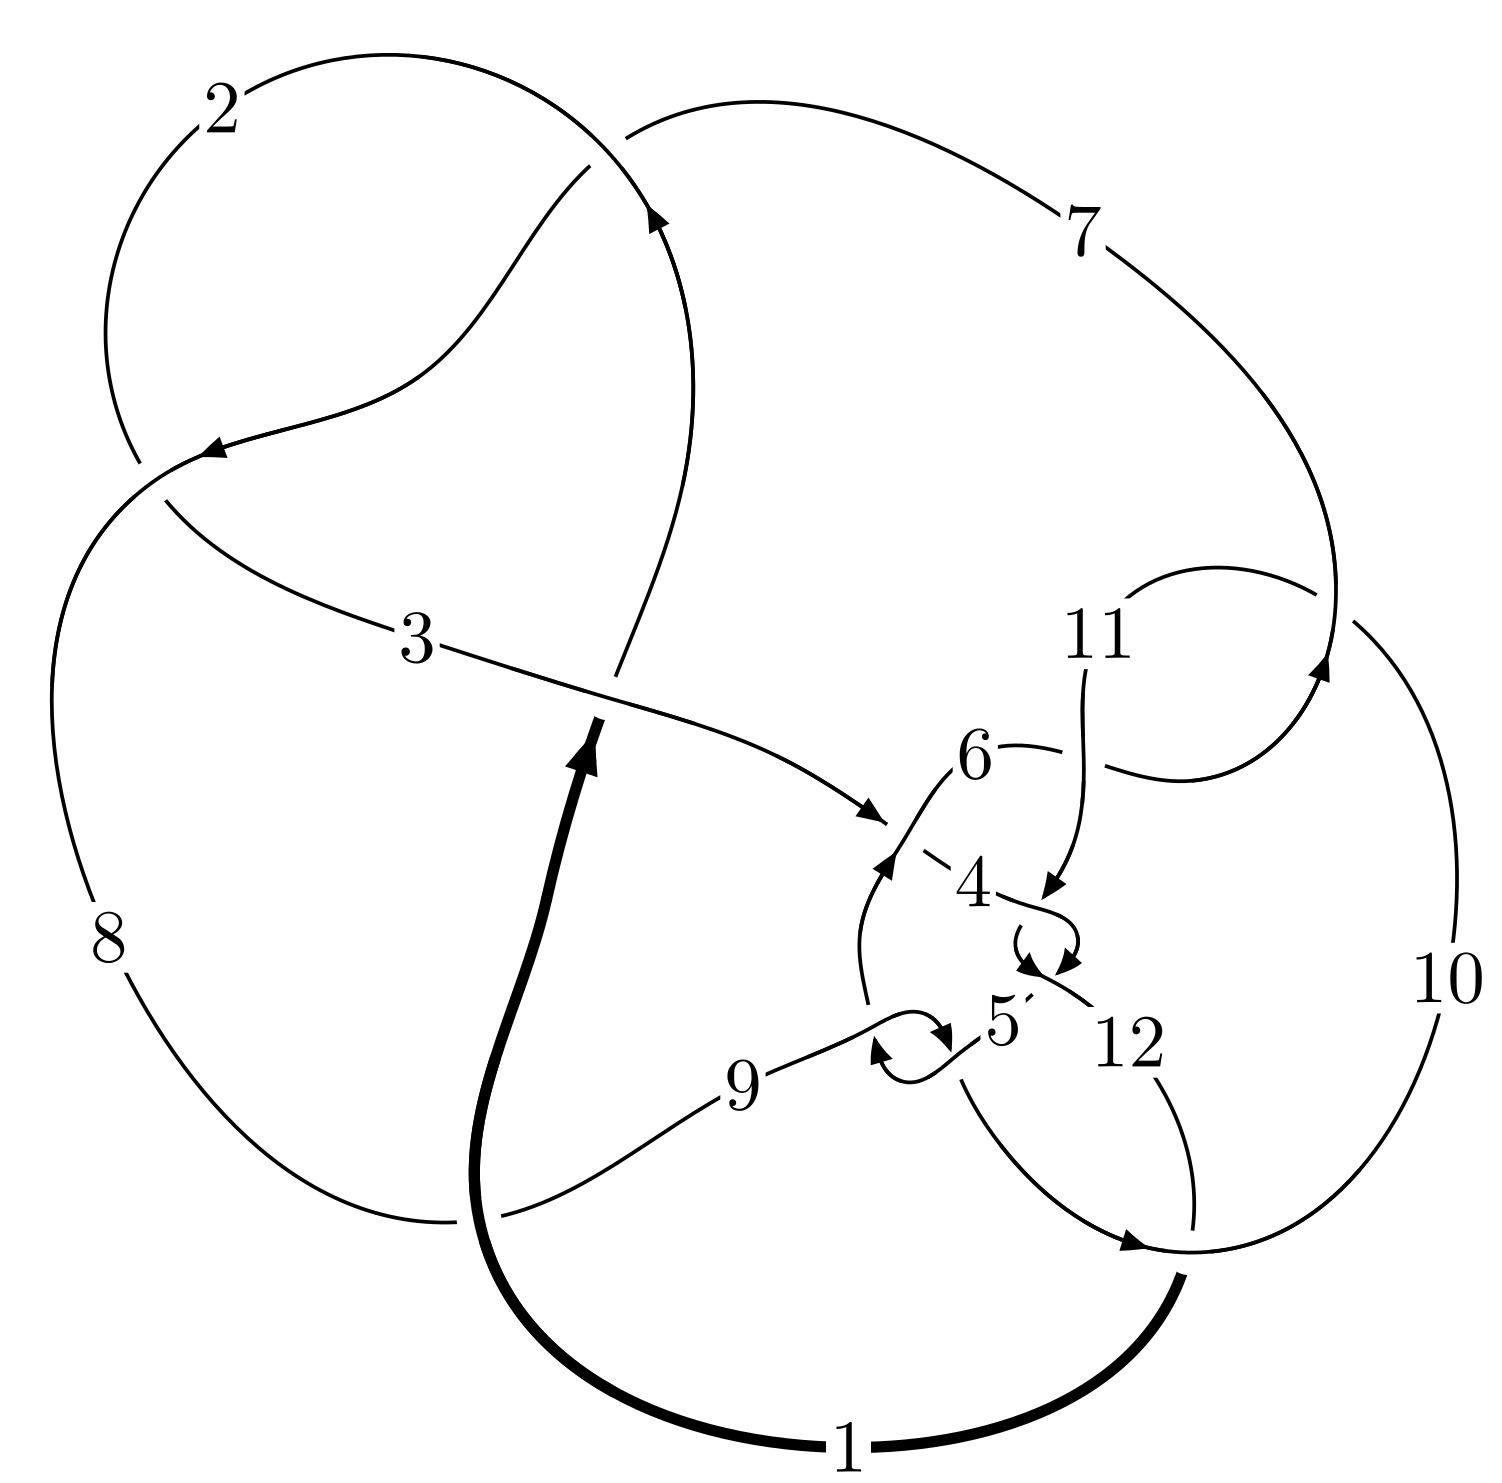
\includegraphics[width=112pt]{../../../GIT/diagram.site/Diagrams/png/1507_12a_0706.png}\\
\ \ \ A knot diagram\footnotemark}&
\allowdisplaybreaks
\textbf{Linearized knot diagam} \\
\cline{2-2}
 &
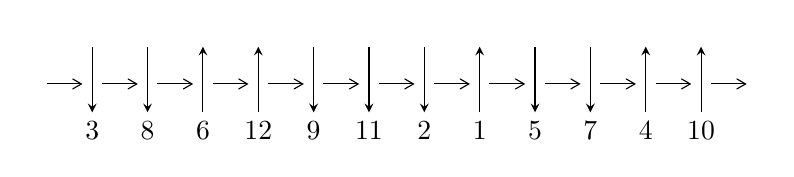
\begin{tikzpicture}[x=20pt, y=17pt]
	% nodes
	\node (C0) at (0, 0) {};
	\node (C1) at (1, 0) {};
	\node (C1U) at (1, +1) {};
	\node (C1D) at (1, -1) {3};

	\node (C2) at (2, 0) {};
	\node (C2U) at (2, +1) {};
	\node (C2D) at (2, -1) {8};

	\node (C3) at (3, 0) {};
	\node (C3U) at (3, +1) {};
	\node (C3D) at (3, -1) {6};

	\node (C4) at (4, 0) {};
	\node (C4U) at (4, +1) {};
	\node (C4D) at (4, -1) {12};

	\node (C5) at (5, 0) {};
	\node (C5U) at (5, +1) {};
	\node (C5D) at (5, -1) {9};

	\node (C6) at (6, 0) {};
	\node (C6U) at (6, +1) {};
	\node (C6D) at (6, -1) {11};

	\node (C7) at (7, 0) {};
	\node (C7U) at (7, +1) {};
	\node (C7D) at (7, -1) {2};

	\node (C8) at (8, 0) {};
	\node (C8U) at (8, +1) {};
	\node (C8D) at (8, -1) {1};

	\node (C9) at (9, 0) {};
	\node (C9U) at (9, +1) {};
	\node (C9D) at (9, -1) {5};

	\node (C10) at (10, 0) {};
	\node (C10U) at (10, +1) {};
	\node (C10D) at (10, -1) {7};

	\node (C11) at (11, 0) {};
	\node (C11U) at (11, +1) {};
	\node (C11D) at (11, -1) {4};

	\node (C12) at (12, 0) {};
	\node (C12U) at (12, +1) {};
	\node (C12D) at (12, -1) {10};
	\node (C13) at (13, 0) {};

	% arrows
	\draw[->,>={angle 60}]
	(C0) edge (C1) (C1) edge (C2) (C2) edge (C3) (C3) edge (C4) (C4) edge (C5) (C5) edge (C6) (C6) edge (C7) (C7) edge (C8) (C8) edge (C9) (C9) edge (C10) (C10) edge (C11) (C11) edge (C12) (C12) edge (C13) ;	\draw[->,>=stealth]
	(C1U) edge (C1D) (C2U) edge (C2D) (C3D) edge (C3U) (C4D) edge (C4U) (C5U) edge (C5D) (C6U) edge (C6D) (C7U) edge (C7D) (C8D) edge (C8U) (C9U) edge (C9D) (C10U) edge (C10D) (C11D) edge (C11U) (C12D) edge (C12U) ;
	\end{tikzpicture} \\
\hhline{~~} \\& 
\textbf{Solving Sequence} \\ \cline{2-2} 
 &
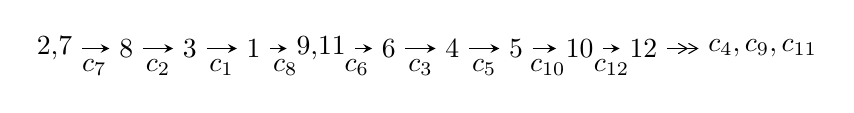
\begin{tikzpicture}[x=23pt, y=7pt]
	% node
	\node (A0) at (-1/8, 0) {2,7};
	\node (A1) at (1, 0) {8};
	\node (A2) at (2, 0) {3};
	\node (A3) at (3, 0) {1};
	\node (A4) at (65/16, 0) {9,11};
	\node (A5) at (41/8, 0) {6};
	\node (A6) at (49/8, 0) {4};
	\node (A7) at (57/8, 0) {5};
	\node (A8) at (65/8, 0) {10};
	\node (A9) at (73/8, 0) {12};
	\node (C1) at (1/2, -1) {$c_{7}$};
	\node (C2) at (3/2, -1) {$c_{2}$};
	\node (C3) at (5/2, -1) {$c_{1}$};
	\node (C4) at (7/2, -1) {$c_{8}$};
	\node (C5) at (37/8, -1) {$c_{6}$};
	\node (C6) at (45/8, -1) {$c_{3}$};
	\node (C7) at (53/8, -1) {$c_{5}$};
	\node (C8) at (61/8, -1) {$c_{10}$};
	\node (C9) at (69/8, -1) {$c_{12}$};
	\node (A10) at (11, 0) {$c_{4},c_{9},c_{11}$};

	% edge
	\draw[->,>=stealth]	
	(A0) edge (A1) (A1) edge (A2) (A2) edge (A3) (A3) edge (A4) (A4) edge (A5) (A5) edge (A6) (A6) edge (A7) (A7) edge (A8) (A8) edge (A9) ;
	\draw[->>,>={angle 60}]	
	(A9) edge (A10);
\end{tikzpicture} \\ 

\end{tabular} \\

\footnotetext{
The image of knot diagram is generated by the software ``\textbf{Draw programme}" developed by Andrew Bartholomew(\url{http://www.layer8.co.uk/maths/draw/index.htm\#Running-draw}), where we modified some parts for our purpose(\url{https://github.com/CATsTAILs/LinksPainter}).
}\phantom \\ \newline 
\centering \textbf{Ideals for irreducible components\footnotemark of $X_{\text{par}}$} 
 
\begin{align*}
I^u_{1}&=\langle 
-8.77122\times10^{31} u^{42}+1.28986\times10^{32} u^{41}+\cdots+6.23372\times10^{32} b-4.00675\times10^{32},\\
\phantom{I^u_{1}}&\phantom{= \langle  }4.66471\times10^{32} u^{42}-7.74777\times10^{32} u^{41}+\cdots+2.49349\times10^{33} a+4.88238\times10^{33},\;u^{43}-3 u^{42}+\cdots-28 u+8\rangle \\
I^u_{2}&=\langle 
-338 u^{34} a+751 u^{34}+\cdots+2112 a-1193,\;90 u^{34} a-8 u^{34}+\cdots+5 a+274,\;u^{35}+u^{34}+\cdots+2 u+1\rangle \\
I^u_{3}&=\langle 
b+1,\;- u^3-4 u^2+4 a+6,\;u^4-2 u^2+2\rangle \\
\\
I^v_{1}&=\langle 
a,\;b-1,\;2 v-1\rangle \\
\end{align*}
\raggedright * 4 irreducible components of $\dim_{\mathbb{C}}=0$, with total 118 representations.\\
\footnotetext{All coefficients of polynomials are rational numbers. But the coefficients are sometimes approximated in decimal forms when there is not enough margin.}
\newpage
\renewcommand{\arraystretch}{1}
\centering \section*{I. $I^u_{1}= \langle -8.77\times10^{31} u^{42}+1.29\times10^{32} u^{41}+\cdots+6.23\times10^{32} b-4.01\times10^{32},\;4.66\times10^{32} u^{42}-7.75\times10^{32} u^{41}+\cdots+2.49\times10^{33} a+4.88\times10^{33},\;u^{43}-3 u^{42}+\cdots-28 u+8 \rangle$}
\flushleft \textbf{(i) Arc colorings}\\
\begin{tabular}{m{7pt} m{180pt} m{7pt} m{180pt} }
\flushright $a_{2}=$&$\begin{pmatrix}0\\u\end{pmatrix}$ \\
\flushright $a_{7}=$&$\begin{pmatrix}1\\0\end{pmatrix}$ \\
\flushright $a_{8}=$&$\begin{pmatrix}1\\u^2\end{pmatrix}$ \\
\flushright $a_{3}=$&$\begin{pmatrix}- u\\- u^3+u\end{pmatrix}$ \\
\flushright $a_{1}=$&$\begin{pmatrix}u^3\\u^5- u^3+u\end{pmatrix}$ \\
\flushright $a_{9}=$&$\begin{pmatrix}u^6- u^4+1\\u^8-2 u^6+2 u^4\end{pmatrix}$ \\
\flushright $a_{11}=$&$\begin{pmatrix}-0.187076 u^{42}+0.310720 u^{41}+\cdots-1.10826 u-1.95805\\0.140706 u^{42}-0.206917 u^{41}+\cdots+0.489729 u+0.642754\end{pmatrix}$ \\
\flushright $a_{6}=$&$\begin{pmatrix}-0.0109355 u^{42}+0.0220436 u^{41}+\cdots-0.0604385 u+0.806906\\-0.00913229 u^{42}-0.0157531 u^{41}+\cdots-0.674511 u+0.907667\end{pmatrix}$ \\
\flushright $a_{4}=$&$\begin{pmatrix}0.0216414 u^{42}-0.0230274 u^{41}+\cdots+0.532942 u-0.0730053\\0.0852608 u^{42}-0.239690 u^{41}+\cdots+2.60820 u-0.0463949\end{pmatrix}$ \\
\flushright $a_{5}=$&$\begin{pmatrix}-0.0643673 u^{42}+0.170970 u^{41}+\cdots-2.78169 u+2.70928\\-0.0198900 u^{42}-0.0117962 u^{41}+\cdots-0.613345 u+0.548201\end{pmatrix}$ \\
\flushright $a_{10}=$&$\begin{pmatrix}-0.0463696 u^{42}+0.103803 u^{41}+\cdots-0.618528 u-1.31530\\0.140706 u^{42}-0.206917 u^{41}+\cdots+0.489729 u+0.642754\end{pmatrix}$ \\
\flushright $a_{12}=$&$\begin{pmatrix}-0.157589 u^{42}+0.303639 u^{41}+\cdots-3.64692 u+0.181125\\0.0870361 u^{42}-0.136522 u^{41}+\cdots+1.11816 u+0.638551\end{pmatrix}$\\&\end{tabular}
\flushleft \textbf{(ii) Obstruction class $= -1$}\\~\\
\flushleft \textbf{(iii) Cusp Shapes $= 0.255497 u^{42}-0.304541 u^{41}+\cdots+16.6870 u+2.47466$}\\~\\
\newpage\renewcommand{\arraystretch}{1}
\flushleft \textbf{(iv) u-Polynomials at the component}\newline \\
\begin{tabular}{m{50pt}|m{274pt}}
Crossings & \hspace{64pt}u-Polynomials at each crossing \\
\hline $$\begin{aligned}c_{1}\end{aligned}$$&$\begin{aligned}
&u^{43}+21 u^{42}+\cdots+272 u+64
\end{aligned}$\\
\hline $$\begin{aligned}c_{2},c_{7}\end{aligned}$$&$\begin{aligned}
&u^{43}-3 u^{42}+\cdots-28 u+8
\end{aligned}$\\
\hline $$\begin{aligned}c_{3},c_{12}\end{aligned}$$&$\begin{aligned}
&128(128 u^{43}+576 u^{42}+\cdots+u+1)
\end{aligned}$\\
\hline $$\begin{aligned}c_{4},c_{11}\end{aligned}$$&$\begin{aligned}
&u^{43}-18 u^{41}+\cdots+889 u+416
\end{aligned}$\\
\hline $$\begin{aligned}c_{5},c_{6},c_{9}\\c_{10}\end{aligned}$$&$\begin{aligned}
&u^{43}- u^{42}+\cdots-24 u+5
\end{aligned}$\\
\hline $$\begin{aligned}c_{8}\end{aligned}$$&$\begin{aligned}
&u^{43}-9 u^{42}+\cdots+2332 u+2968
\end{aligned}$\\
\hline
\end{tabular}\\~\\
\newpage\renewcommand{\arraystretch}{1}
\flushleft \textbf{(v) Riley Polynomials at the component}\newline \\
\begin{tabular}{m{50pt}|m{274pt}}
Crossings & \hspace{64pt}Riley Polynomials at each crossing \\
\hline $$\begin{aligned}c_{1}\end{aligned}$$&$\begin{aligned}
&y^{43}+3 y^{42}+\cdots-36608 y-4096
\end{aligned}$\\
\hline $$\begin{aligned}c_{2},c_{7}\end{aligned}$$&$\begin{aligned}
&y^{43}-21 y^{42}+\cdots+272 y-64
\end{aligned}$\\
\hline $$\begin{aligned}c_{3},c_{12}\end{aligned}$$&$\begin{aligned}
&16384(16384 y^{43}-274432 y^{42}+\cdots+75 y-1)
\end{aligned}$\\
\hline $$\begin{aligned}c_{4},c_{11}\end{aligned}$$&$\begin{aligned}
&y^{43}-36 y^{42}+\cdots+989169 y-173056
\end{aligned}$\\
\hline $$\begin{aligned}c_{5},c_{6},c_{9}\\c_{10}\end{aligned}$$&$\begin{aligned}
&y^{43}+19 y^{42}+\cdots+126 y-25
\end{aligned}$\\
\hline $$\begin{aligned}c_{8}\end{aligned}$$&$\begin{aligned}
&y^{43}+15 y^{42}+\cdots+81561488 y-8809024
\end{aligned}$\\
\hline
\end{tabular}\\~\\
\newpage\flushleft \textbf{(vi) Complex Volumes and Cusp Shapes}
$$\begin{array}{c|c|c}  
\text{Solutions to }I^u_{1}& \I (\text{vol} + \sqrt{-1}CS) & \text{Cusp shape}\\
 \hline 
\begin{aligned}
u &= -0.364395 + 0.877924 I \\
a &= \phantom{-}0.04638 - 1.82403 I \\
b &= \phantom{-}0.391782 + 1.198260 I\end{aligned}
 & \phantom{-}4.01698 - 7.46652 I & \phantom{-}3.11751 + 6.34023 I \\ \hline\begin{aligned}
u &= -0.364395 - 0.877924 I \\
a &= \phantom{-}0.04638 + 1.82403 I \\
b &= \phantom{-}0.391782 - 1.198260 I\end{aligned}
 & \phantom{-}4.01698 + 7.46652 I & \phantom{-}3.11751 - 6.34023 I \\ \hline\begin{aligned}
u &= \phantom{-}0.756742 + 0.762090 I \\
a &= \phantom{-}0.61467 - 2.10710 I \\
b &= \phantom{-}0.38983 + 1.39078 I\end{aligned}
 & \phantom{-}12.3032 - 10.3019 I & \phantom{-}6.09134 + 7.29034 I \\ \hline\begin{aligned}
u &= \phantom{-}0.756742 - 0.762090 I \\
a &= \phantom{-}0.61467 + 2.10710 I \\
b &= \phantom{-}0.38983 - 1.39078 I\end{aligned}
 & \phantom{-}12.3032 + 10.3019 I & \phantom{-}6.09134 - 7.29034 I \\ \hline\begin{aligned}
u &= \phantom{-}0.309821 + 0.864620 I \\
a &= \phantom{-}0.23217 + 1.87818 I \\
b &= \phantom{-}0.54746 - 1.38673 I\end{aligned}
 & \phantom{-}9.6780 + 13.4175 I & \phantom{-}4.66358 - 6.56976 I \\ \hline\begin{aligned}
u &= \phantom{-}0.309821 - 0.864620 I \\
a &= \phantom{-}0.23217 - 1.87818 I \\
b &= \phantom{-}0.54746 + 1.38673 I\end{aligned}
 & \phantom{-}9.6780 - 13.4175 I & \phantom{-}4.66358 + 6.56976 I \\ \hline\begin{aligned}
u &= \phantom{-}0.263698 + 1.077760 I \\
a &= \phantom{-}0.063581 + 1.403550 I \\
b &= -0.030867 - 1.141810 I\end{aligned}
 & \phantom{-}7.30362 - 1.07498 I & \phantom{-}16.0017 + 3.6754 I \\ \hline\begin{aligned}
u &= \phantom{-}0.263698 - 1.077760 I \\
a &= \phantom{-}0.063581 - 1.403550 I \\
b &= -0.030867 + 1.141810 I\end{aligned}
 & \phantom{-}7.30362 + 1.07498 I & \phantom{-}16.0017 - 3.6754 I \\ \hline\begin{aligned}
u &= -1.045620 + 0.374301 I \\
a &= \phantom{-}1.32312 + 1.26742 I \\
b &= \phantom{-}1.240050 - 0.457624 I\end{aligned}
 & -2.30003 + 1.95260 I & -1.79739 + 0.90426 I \\ \hline\begin{aligned}
u &= -1.045620 - 0.374301 I \\
a &= \phantom{-}1.32312 - 1.26742 I \\
b &= \phantom{-}1.240050 + 0.457624 I\end{aligned}
 & -2.30003 - 1.95260 I & -1.79739 - 0.90426 I\\
 \hline 
 \end{array}$$\newpage$$\begin{array}{c|c|c}  
\text{Solutions to }I^u_{1}& \I (\text{vol} + \sqrt{-1}CS) & \text{Cusp shape}\\
 \hline 
\begin{aligned}
u &= \phantom{-}1.044540 + 0.384315 I \\
a &= \phantom{-}0.304099 + 0.657915 I \\
b &= -0.100329 - 0.404925 I\end{aligned}
 & -0.22935 - 3.67460 I & -0.89632 + 6.35112 I \\ \hline\begin{aligned}
u &= \phantom{-}1.044540 - 0.384315 I \\
a &= \phantom{-}0.304099 - 0.657915 I \\
b &= -0.100329 + 0.404925 I\end{aligned}
 & -0.22935 + 3.67460 I & -0.89632 - 6.35112 I \\ \hline\begin{aligned}
u &= -0.846910 + 0.182966 I \\
a &= \phantom{-}0.062155 + 0.638512 I \\
b &= -0.715260 - 0.471235 I\end{aligned}
 & -0.998880 + 0.351600 I & -6.01917 - 1.74255 I \\ \hline\begin{aligned}
u &= -0.846910 - 0.182966 I \\
a &= \phantom{-}0.062155 - 0.638512 I \\
b &= -0.715260 + 0.471235 I\end{aligned}
 & -0.998880 - 0.351600 I & -6.01917 + 1.74255 I \\ \hline\begin{aligned}
u &= \phantom{-}0.867602 + 0.745647 I \\
a &= \phantom{-}0.99486 - 1.48397 I \\
b &= -0.307161 + 1.363000 I\end{aligned}
 & \phantom{-}11.98760 + 4.69062 I & \phantom{-}6.27466 - 2.28196 I \\ \hline\begin{aligned}
u &= \phantom{-}0.867602 - 0.745647 I \\
a &= \phantom{-}0.99486 + 1.48397 I \\
b &= -0.307161 - 1.363000 I\end{aligned}
 & \phantom{-}11.98760 - 4.69062 I & \phantom{-}6.27466 + 2.28196 I \\ \hline\begin{aligned}
u &= \phantom{-}1.079400 + 0.517359 I \\
a &= -0.01844 - 1.52789 I \\
b &= \phantom{-}1.49377 - 0.29947 I\end{aligned}
 & -1.25135 - 4.90293 I & \phantom{-}2.46086 + 7.07158 I \\ \hline\begin{aligned}
u &= \phantom{-}1.079400 - 0.517359 I \\
a &= -0.01844 + 1.52789 I \\
b &= \phantom{-}1.49377 + 0.29947 I\end{aligned}
 & -1.25135 + 4.90293 I & \phantom{-}2.46086 - 7.07158 I \\ \hline\begin{aligned}
u &= -0.790225 + 0.907782 I \\
a &= \phantom{-}0.45900 + 1.60463 I \\
b &= \phantom{-}0.082408 - 1.150310 I\end{aligned}
 & \phantom{-}6.23041 + 3.24342 I & \phantom{-}11.79096 - 7.78462 I \\ \hline\begin{aligned}
u &= -0.790225 - 0.907782 I \\
a &= \phantom{-}0.45900 - 1.60463 I \\
b &= \phantom{-}0.082408 + 1.150310 I\end{aligned}
 & \phantom{-}6.23041 - 3.24342 I & \phantom{-}11.79096 + 7.78462 I\\
 \hline 
 \end{array}$$\newpage$$\begin{array}{c|c|c}  
\text{Solutions to }I^u_{1}& \I (\text{vol} + \sqrt{-1}CS) & \text{Cusp shape}\\
 \hline 
\begin{aligned}
u &= \phantom{-}1.136540 + 0.399301 I \\
a &= \phantom{-}1.014030 - 0.675093 I \\
b &= \phantom{-}0.799216 + 0.538229 I\end{aligned}
 & -4.92648 - 4.54280 I & -9.30891 + 6.68648 I \\ \hline\begin{aligned}
u &= \phantom{-}1.136540 - 0.399301 I \\
a &= \phantom{-}1.014030 + 0.675093 I \\
b &= \phantom{-}0.799216 - 0.538229 I\end{aligned}
 & -4.92648 + 4.54280 I & -9.30891 - 6.68648 I \\ \hline\begin{aligned}
u &= \phantom{-}1.217380 + 0.123691 I \\
a &= -0.278389 - 0.273065 I \\
b &= -0.417369 + 1.014720 I\end{aligned}
 & -1.53276 + 4.52647 I & -3.84680 - 6.77592 I \\ \hline\begin{aligned}
u &= \phantom{-}1.217380 - 0.123691 I \\
a &= -0.278389 + 0.273065 I \\
b &= -0.417369 - 1.014720 I\end{aligned}
 & -1.53276 - 4.52647 I & -3.84680 + 6.77592 I \\ \hline\begin{aligned}
u &= -1.127830 + 0.474826 I \\
a &= \phantom{-}0.096382 + 0.762504 I \\
b &= \phantom{-}0.864085 + 0.359880 I\end{aligned}
 & -4.41300 + 3.28480 I & -9.46585 - 1.64947 I \\ \hline\begin{aligned}
u &= -1.127830 - 0.474826 I \\
a &= \phantom{-}0.096382 - 0.762504 I \\
b &= \phantom{-}0.864085 - 0.359880 I\end{aligned}
 & -4.41300 - 3.28480 I & -9.46585 + 1.64947 I \\ \hline\begin{aligned}
u &= -1.238660 + 0.218673 I \\
a &= -0.381217 - 0.075299 I \\
b &= -0.53587 - 1.30966 I\end{aligned}
 & \phantom{-}4.54892 - 10.07780 I & -0.39399 + 5.36382 I \\ \hline\begin{aligned}
u &= -1.238660 - 0.218673 I \\
a &= -0.381217 + 0.075299 I \\
b &= -0.53587 + 1.30966 I\end{aligned}
 & \phantom{-}4.54892 + 10.07780 I & -0.39399 - 5.36382 I \\ \hline\begin{aligned}
u &= -1.153790 + 0.610907 I \\
a &= -1.48361 - 1.48093 I \\
b &= -0.458133 + 1.229980 I\end{aligned}
 & \phantom{-}1.62850 + 12.94670 I & \phantom{-0.000000 } 0. - 9.56767 I \\ \hline\begin{aligned}
u &= -1.153790 - 0.610907 I \\
a &= -1.48361 + 1.48093 I \\
b &= -0.458133 - 1.229980 I\end{aligned}
 & \phantom{-}1.62850 - 12.94670 I & \phantom{-0.000000 -}0. + 9.56767 I\\
 \hline 
 \end{array}$$\newpage$$\begin{array}{c|c|c}  
\text{Solutions to }I^u_{1}& \I (\text{vol} + \sqrt{-1}CS) & \text{Cusp shape}\\
 \hline 
\begin{aligned}
u &= -0.694049\phantom{ +0.000000I} \\
a &= -0.0645283\phantom{ +0.000000I} \\
b &= -0.550881\phantom{ +0.000000I}\end{aligned}
 & -1.02637\phantom{ +0.000000I} & -10.0280\phantom{ +0.000000I} \\ \hline\begin{aligned}
u &= \phantom{-}1.167800 + 0.591087 I \\
a &= -1.86194 + 1.44933 I \\
b &= -0.58874 - 1.39305 I\end{aligned}
 & \phantom{-}7.1025 - 18.7791 I & \phantom{-}1.67063 + 10.13873 I \\ \hline\begin{aligned}
u &= \phantom{-}1.167800 - 0.591087 I \\
a &= -1.86194 - 1.44933 I \\
b &= -0.58874 + 1.39305 I\end{aligned}
 & \phantom{-}7.1025 + 18.7791 I & \phantom{-}1.67063 - 10.13873 I \\ \hline\begin{aligned}
u &= \phantom{-}0.370173 + 0.562820 I \\
a &= \phantom{-}0.890218 + 0.191663 I \\
b &= -1.40761 - 0.15779 I\end{aligned}
 & \phantom{-}0.787413 + 0.515759 I & \phantom{-}8.15856 - 2.76240 I \\ \hline\begin{aligned}
u &= \phantom{-}0.370173 - 0.562820 I \\
a &= \phantom{-}0.890218 - 0.191663 I \\
b &= -1.40761 + 0.15779 I\end{aligned}
 & \phantom{-}0.787413 - 0.515759 I & \phantom{-}8.15856 + 2.76240 I \\ \hline\begin{aligned}
u &= -0.085379 + 0.627851 I \\
a &= \phantom{-}0.241341 - 0.446824 I \\
b &= -0.728213 + 0.394310 I\end{aligned}
 & -1.60222 + 0.88694 I & -6.18860 - 3.12820 I \\ \hline\begin{aligned}
u &= -0.085379 - 0.627851 I \\
a &= \phantom{-}0.241341 + 0.446824 I \\
b &= -0.728213 - 0.394310 I\end{aligned}
 & -1.60222 - 0.88694 I & -6.18860 + 3.12820 I \\ \hline\begin{aligned}
u &= \phantom{-}1.208770 + 0.701017 I \\
a &= -0.901694 + 1.038270 I \\
b &= -0.114387 - 1.123360 I\end{aligned}
 & \phantom{-}4.48482 - 5.24026 I & \phantom{-}9.16270 + 10.48846 I \\ \hline\begin{aligned}
u &= \phantom{-}1.208770 - 0.701017 I \\
a &= -0.901694 - 1.038270 I \\
b &= -0.114387 + 1.123360 I\end{aligned}
 & \phantom{-}4.48482 + 5.24026 I & \phantom{-}9.16270 - 10.48846 I \\ \hline\begin{aligned}
u &= -1.342780 + 0.405991 I \\
a &= \phantom{-}0.590693 + 0.381161 I \\
b &= \phantom{-}0.193810 - 1.053580 I\end{aligned}
 & \phantom{-}2.11212 + 6.10939 I & \phantom{-0.000000 } 0. - 12.47941 I\\
 \hline 
 \end{array}$$\newpage$$\begin{array}{c|c|c}  
\text{Solutions to }I^u_{1}& \I (\text{vol} + \sqrt{-1}CS) & \text{Cusp shape}\\
 \hline 
\begin{aligned}
u &= -1.342780 - 0.405991 I \\
a &= \phantom{-}0.590693 - 0.381161 I \\
b &= \phantom{-}0.193810 + 1.053580 I\end{aligned}
 & \phantom{-}2.11212 - 6.10939 I & \phantom{-0.000000 -}0. + 12.47941 I \\ \hline\begin{aligned}
u &= \phantom{-}0.420151 + 0.385137 I \\
a &= -1.47515 + 0.40144 I \\
b &= \phantom{-}0.176966 - 0.117588 I\end{aligned}
 & \phantom{-}1.51091 + 0.21948 I & \phantom{-}6.61608 - 0.74738 I \\ \hline\begin{aligned}
u &= \phantom{-}0.420151 - 0.385137 I \\
a &= -1.47515 - 0.40144 I \\
b &= \phantom{-}0.176966 + 0.117588 I\end{aligned}
 & \phantom{-}1.51091 - 0.21948 I & \phantom{-}6.61608 + 0.74738 I\\
 \hline 
 \end{array}$$\newpage\newpage\renewcommand{\arraystretch}{1}
\centering \section*{II. $I^u_{2}= \langle -338 u^{34} a+751 u^{34}+\cdots+2112 a-1193,\;90 u^{34} a-8 u^{34}+\cdots+5 a+274,\;u^{35}+u^{34}+\cdots+2 u+1 \rangle$}
\flushleft \textbf{(i) Arc colorings}\\
\begin{tabular}{m{7pt} m{180pt} m{7pt} m{180pt} }
\flushright $a_{2}=$&$\begin{pmatrix}0\\u\end{pmatrix}$ \\
\flushright $a_{7}=$&$\begin{pmatrix}1\\0\end{pmatrix}$ \\
\flushright $a_{8}=$&$\begin{pmatrix}1\\u^2\end{pmatrix}$ \\
\flushright $a_{3}=$&$\begin{pmatrix}- u\\- u^3+u\end{pmatrix}$ \\
\flushright $a_{1}=$&$\begin{pmatrix}u^3\\u^5- u^3+u\end{pmatrix}$ \\
\flushright $a_{9}=$&$\begin{pmatrix}u^6- u^4+1\\u^8-2 u^6+2 u^4\end{pmatrix}$ \\
\flushright $a_{11}=$&$\begin{pmatrix}a\\0.0725789 a u^{34}-0.161263 u^{34}+\cdots-0.453511 a+0.256174\end{pmatrix}$ \\
\flushright $a_{6}=$&$\begin{pmatrix}-0.161263 a u^{34}+1.98020 u^{34}+\cdots+0.256174 a-0.298776\\0.120464 a u^{34}+0.0725789 u^{34}+\cdots+0.0283444 a+0.546489\end{pmatrix}$ \\
\flushright $a_{4}=$&$\begin{pmatrix}-2.63629 a u^{34}-1.29937 u^{34}+\cdots-0.973245 a-4.98809\\0.000858922 a u^{34}-2.41374 u^{34}+\cdots-0.0586214 a-0.862057\end{pmatrix}$ \\
\flushright $a_{5}=$&$\begin{pmatrix}-0.161263 a u^{34}+1.98020 u^{34}+\cdots+0.256174 a-1.29878\\1\end{pmatrix}$ \\
\flushright $a_{10}=$&$\begin{pmatrix}0.0725789 a u^{34}-0.161263 u^{34}+\cdots+0.546489 a+0.256174\\0.0725789 a u^{34}-0.161263 u^{34}+\cdots-0.453511 a+0.256174\end{pmatrix}$ \\
\flushright $a_{12}=$&$\begin{pmatrix}-2.41374 a u^{34}-0.700116 u^{34}+\cdots-0.862057 a-2.24709\\0.439768 a u^{34}-2.63629 u^{34}+\cdots-0.0141722 a-0.973245\end{pmatrix}$\\&\end{tabular}
\flushleft \textbf{(ii) Obstruction class $= -1$}\\~\\
\flushleft \textbf{(iii) Cusp Shapes $= 4 u^{33}-32 u^{31}-4 u^{30}+132 u^{29}+28 u^{28}-348 u^{27}-100 u^{26}+644 u^{25}+224 u^{24}-868 u^{23}-344 u^{22}+880 u^{21}+376 u^{20}-700 u^{19}-312 u^{18}+488 u^{17}+228 u^{16}-336 u^{15}-180 u^{14}+232 u^{13}+140 u^{12}-136 u^{11}-88 u^{10}+72 u^9+44 u^8-32 u^7-24 u^6+16 u^5+16 u^4-4 u^3-8 u^2+6$}\\~\\
\newpage\renewcommand{\arraystretch}{1}
\flushleft \textbf{(iv) u-Polynomials at the component}\newline \\
\begin{tabular}{m{50pt}|m{274pt}}
Crossings & \hspace{64pt}u-Polynomials at each crossing \\
\hline $$\begin{aligned}c_{1}\end{aligned}$$&$\begin{aligned}
&(u^{35}+17 u^{34}+\cdots+2 u+1)^{2}
\end{aligned}$\\
\hline $$\begin{aligned}c_{2},c_{7}\end{aligned}$$&$\begin{aligned}
&(u^{35}+u^{34}+\cdots+2 u+1)^{2}
\end{aligned}$\\
\hline $$\begin{aligned}c_{3},c_{12}\end{aligned}$$&$\begin{aligned}
&25(25 u^{70}-165 u^{69}+\cdots+4.75915\times10^{8} u+3.82582\times10^{7})
\end{aligned}$\\
\hline $$\begin{aligned}c_{4},c_{11}\end{aligned}$$&$\begin{aligned}
&(u^{35}- u^{34}+\cdots+u^2-1)^{2}
\end{aligned}$\\
\hline $$\begin{aligned}c_{5},c_{6},c_{9}\\c_{10}\end{aligned}$$&$\begin{aligned}
&u^{70}+3 u^{69}+\cdots+8 u+1
\end{aligned}$\\
\hline $$\begin{aligned}c_{8}\end{aligned}$$&$\begin{aligned}
&(u^{35}+3 u^{34}+\cdots+58 u+7)^{2}
\end{aligned}$\\
\hline
\end{tabular}\\~\\
\newpage\renewcommand{\arraystretch}{1}
\flushleft \textbf{(v) Riley Polynomials at the component}\newline \\
\begin{tabular}{m{50pt}|m{274pt}}
Crossings & \hspace{64pt}Riley Polynomials at each crossing \\
\hline $$\begin{aligned}c_{1}\end{aligned}$$&$\begin{aligned}
&(y^{35}+3 y^{34}+\cdots-14 y-1)^{2}
\end{aligned}$\\
\hline $$\begin{aligned}c_{2},c_{7}\end{aligned}$$&$\begin{aligned}
&(y^{35}-17 y^{34}+\cdots+2 y-1)^{2}
\end{aligned}$\\
\hline $$\begin{aligned}c_{3},c_{12}\end{aligned}$$&$\begin{aligned}
&625(625 y^{70}-23125 y^{69}+\cdots-1.79208\times10^{16} y+1.46369\times10^{15})
\end{aligned}$\\
\hline $$\begin{aligned}c_{4},c_{11}\end{aligned}$$&$\begin{aligned}
&(y^{35}-29 y^{34}+\cdots+2 y-1)^{2}
\end{aligned}$\\
\hline $$\begin{aligned}c_{5},c_{6},c_{9}\\c_{10}\end{aligned}$$&$\begin{aligned}
&y^{70}+47 y^{69}+\cdots+16 y+1
\end{aligned}$\\
\hline $$\begin{aligned}c_{8}\end{aligned}$$&$\begin{aligned}
&(y^{35}+11 y^{34}+\cdots+1446 y-49)^{2}
\end{aligned}$\\
\hline
\end{tabular}\\~\\
\newpage\flushleft \textbf{(vi) Complex Volumes and Cusp Shapes}
$$\begin{array}{c|c|c}  
\text{Solutions to }I^u_{2}& \I (\text{vol} + \sqrt{-1}CS) & \text{Cusp shape}\\
 \hline 
\begin{aligned}
u &= -0.890522 + 0.542191 I \\
a &= \phantom{-}0.420148 - 1.134650 I \\
b &= -0.887010 - 0.496104 I\end{aligned}
 & \phantom{-}6.32924 - 0.83862 I & \phantom{-}3.46140 - 0.32367 I \\ \hline\begin{aligned}
u &= -0.890522 + 0.542191 I \\
a &= -1.81892 - 1.34506 I \\
b &= \phantom{-}0.17214 + 1.46425 I\end{aligned}
 & \phantom{-}6.32924 - 0.83862 I & \phantom{-}3.46140 - 0.32367 I \\ \hline\begin{aligned}
u &= -0.890522 - 0.542191 I \\
a &= \phantom{-}0.420148 + 1.134650 I \\
b &= -0.887010 + 0.496104 I\end{aligned}
 & \phantom{-}6.32924 + 0.83862 I & \phantom{-}3.46140 + 0.32367 I \\ \hline\begin{aligned}
u &= -0.890522 - 0.542191 I \\
a &= -1.81892 + 1.34506 I \\
b &= \phantom{-}0.17214 - 1.46425 I\end{aligned}
 & \phantom{-}6.32924 + 0.83862 I & \phantom{-}3.46140 + 0.32367 I \\ \hline\begin{aligned}
u &= \phantom{-}0.996188 + 0.423828 I \\
a &= -0.787246 + 0.845478 I \\
b &= -0.352524 + 0.767455 I\end{aligned}
 & \phantom{-}1.75221 - 1.71623 I & -3.26691 - 0.12597 I \\ \hline\begin{aligned}
u &= \phantom{-}0.996188 + 0.423828 I \\
a &= -1.23437 + 1.84232 I \\
b &= -0.064633 - 1.226040 I\end{aligned}
 & \phantom{-}1.75221 - 1.71623 I & -3.26691 - 0.12597 I \\ \hline\begin{aligned}
u &= \phantom{-}0.996188 - 0.423828 I \\
a &= -0.787246 - 0.845478 I \\
b &= -0.352524 - 0.767455 I\end{aligned}
 & \phantom{-}1.75221 + 1.71623 I & -3.26691 + 0.12597 I \\ \hline\begin{aligned}
u &= \phantom{-}0.996188 - 0.423828 I \\
a &= -1.23437 - 1.84232 I \\
b &= -0.064633 + 1.226040 I\end{aligned}
 & \phantom{-}1.75221 + 1.71623 I & -3.26691 + 0.12597 I \\ \hline\begin{aligned}
u &= -0.665614 + 0.623440 I \\
a &= -0.439114 + 0.434345 I \\
b &= \phantom{-}1.033840 - 0.288357 I\end{aligned}
 & \phantom{-}6.99216 + 5.45820 I & \phantom{-}4.60996 - 5.96309 I \\ \hline\begin{aligned}
u &= -0.665614 + 0.623440 I \\
a &= -0.40352 - 2.35368 I \\
b &= -0.34875 + 1.47367 I\end{aligned}
 & \phantom{-}6.99216 + 5.45820 I & \phantom{-}4.60996 - 5.96309 I\\
 \hline 
 \end{array}$$\newpage$$\begin{array}{c|c|c}  
\text{Solutions to }I^u_{2}& \I (\text{vol} + \sqrt{-1}CS) & \text{Cusp shape}\\
 \hline 
\begin{aligned}
u &= -0.665614 - 0.623440 I \\
a &= -0.439114 - 0.434345 I \\
b &= \phantom{-}1.033840 + 0.288357 I\end{aligned}
 & \phantom{-}6.99216 - 5.45820 I & \phantom{-}4.60996 + 5.96309 I \\ \hline\begin{aligned}
u &= -0.665614 - 0.623440 I \\
a &= -0.40352 + 2.35368 I \\
b &= -0.34875 - 1.47367 I\end{aligned}
 & \phantom{-}6.99216 - 5.45820 I & \phantom{-}4.60996 + 5.96309 I \\ \hline\begin{aligned}
u &= -0.903342\phantom{ +0.000000I} \\
a &= -1.89131 + 1.48396 I \\
b &= -0.344219 + 1.164240 I\end{aligned}
 & \phantom{-}5.63430\phantom{ +0.000000I} & \phantom{-}0.141130\phantom{ +0.000000I} \\ \hline\begin{aligned}
u &= -0.903342\phantom{ +0.000000I} \\
a &= -1.89131 - 1.48396 I \\
b &= -0.344219 - 1.164240 I\end{aligned}
 & \phantom{-}5.63430\phantom{ +0.000000I} & \phantom{-}0.141130\phantom{ +0.000000I} \\ \hline\begin{aligned}
u &= \phantom{-}0.688085 + 0.531421 I \\
a &= \phantom{-}0.212009 + 0.451127 I \\
b &= \phantom{-}0.336278 + 0.239728 I\end{aligned}
 & \phantom{-}2.50904 - 2.01862 I & -1.09133 + 4.63726 I \\ \hline\begin{aligned}
u &= \phantom{-}0.688085 + 0.531421 I \\
a &= -0.88597 + 2.22330 I \\
b &= -0.108999 - 1.142220 I\end{aligned}
 & \phantom{-}2.50904 - 2.01862 I & -1.09133 + 4.63726 I \\ \hline\begin{aligned}
u &= \phantom{-}0.688085 - 0.531421 I \\
a &= \phantom{-}0.212009 - 0.451127 I \\
b &= \phantom{-}0.336278 - 0.239728 I\end{aligned}
 & \phantom{-}2.50904 + 2.01862 I & -1.09133 - 4.63726 I \\ \hline\begin{aligned}
u &= \phantom{-}0.688085 - 0.531421 I \\
a &= -0.88597 - 2.22330 I \\
b &= -0.108999 + 1.142220 I\end{aligned}
 & \phantom{-}2.50904 + 2.01862 I & -1.09133 - 4.63726 I \\ \hline\begin{aligned}
u &= -1.059800 + 0.502369 I \\
a &= \phantom{-}0.26147 + 1.61880 I \\
b &= -0.234288 - 1.162630 I\end{aligned}
 & \phantom{-}2.48084 + 4.67146 I & -0.51273 - 7.37463 I \\ \hline\begin{aligned}
u &= -1.059800 + 0.502369 I \\
a &= -2.79747 - 1.54656 I \\
b &= -0.319958 + 1.048700 I\end{aligned}
 & \phantom{-}2.48084 + 4.67146 I & -0.51273 - 7.37463 I\\
 \hline 
 \end{array}$$\newpage$$\begin{array}{c|c|c}  
\text{Solutions to }I^u_{2}& \I (\text{vol} + \sqrt{-1}CS) & \text{Cusp shape}\\
 \hline 
\begin{aligned}
u &= -1.059800 - 0.502369 I \\
a &= \phantom{-}0.26147 - 1.61880 I \\
b &= -0.234288 + 1.162630 I\end{aligned}
 & \phantom{-}2.48084 - 4.67146 I & -0.51273 + 7.37463 I \\ \hline\begin{aligned}
u &= -1.059800 - 0.502369 I \\
a &= -2.79747 + 1.54656 I \\
b &= -0.319958 - 1.048700 I\end{aligned}
 & \phantom{-}2.48084 - 4.67146 I & -0.51273 + 7.37463 I \\ \hline\begin{aligned}
u &= \phantom{-}1.146120 + 0.254789 I \\
a &= -1.037470 + 0.622193 I \\
b &= -1.044800 - 0.117101 I\end{aligned}
 & \phantom{-}0.76959 + 4.45397 I & -3.15239 - 2.81525 I \\ \hline\begin{aligned}
u &= \phantom{-}1.146120 + 0.254789 I \\
a &= \phantom{-}0.169760 - 0.407579 I \\
b &= \phantom{-}0.59055 - 1.28795 I\end{aligned}
 & \phantom{-}0.76959 + 4.45397 I & -3.15239 - 2.81525 I \\ \hline\begin{aligned}
u &= \phantom{-}1.146120 - 0.254789 I \\
a &= -1.037470 - 0.622193 I \\
b &= -1.044800 + 0.117101 I\end{aligned}
 & \phantom{-}0.76959 - 4.45397 I & -3.15239 + 2.81525 I \\ \hline\begin{aligned}
u &= \phantom{-}1.146120 - 0.254789 I \\
a &= \phantom{-}0.169760 + 0.407579 I \\
b &= \phantom{-}0.59055 + 1.28795 I\end{aligned}
 & \phantom{-}0.76959 - 4.45397 I & -3.15239 + 2.81525 I \\ \hline\begin{aligned}
u &= -0.308085 + 0.766136 I \\
a &= -0.588916 - 0.042005 I \\
b &= \phantom{-}1.177980 + 0.012281 I\end{aligned}
 & \phantom{-}5.25576 - 7.38977 I & \phantom{-}3.01566 + 5.00078 I \\ \hline\begin{aligned}
u &= -0.308085 + 0.766136 I \\
a &= -0.10013 + 1.93999 I \\
b &= -0.58139 - 1.43466 I\end{aligned}
 & \phantom{-}5.25576 - 7.38977 I & \phantom{-}3.01566 + 5.00078 I \\ \hline\begin{aligned}
u &= -0.308085 - 0.766136 I \\
a &= -0.588916 + 0.042005 I \\
b &= \phantom{-}1.177980 - 0.012281 I\end{aligned}
 & \phantom{-}5.25576 + 7.38977 I & \phantom{-}3.01566 - 5.00078 I \\ \hline\begin{aligned}
u &= -0.308085 - 0.766136 I \\
a &= -0.10013 - 1.93999 I \\
b &= -0.58139 + 1.43466 I\end{aligned}
 & \phantom{-}5.25576 + 7.38977 I & \phantom{-}3.01566 - 5.00078 I\\
 \hline 
 \end{array}$$\newpage$$\begin{array}{c|c|c}  
\text{Solutions to }I^u_{2}& \I (\text{vol} + \sqrt{-1}CS) & \text{Cusp shape}\\
 \hline 
\begin{aligned}
u &= -1.142990 + 0.287310 I \\
a &= -0.674948 - 0.484137 I \\
b &= -0.687825 + 0.345199 I\end{aligned}
 & -3.52386 - 0.30557 I & -7.68573 + 0.05854 I \\ \hline\begin{aligned}
u &= -1.142990 + 0.287310 I \\
a &= \phantom{-}0.277824 + 0.046595 I \\
b &= \phantom{-}0.500699 + 0.963199 I\end{aligned}
 & -3.52386 - 0.30557 I & -7.68573 + 0.05854 I \\ \hline\begin{aligned}
u &= -1.142990 - 0.287310 I \\
a &= -0.674948 + 0.484137 I \\
b &= -0.687825 - 0.345199 I\end{aligned}
 & -3.52386 + 0.30557 I & -7.68573 - 0.05854 I \\ \hline\begin{aligned}
u &= -1.142990 - 0.287310 I \\
a &= \phantom{-}0.277824 - 0.046595 I \\
b &= \phantom{-}0.500699 - 0.963199 I\end{aligned}
 & -3.52386 + 0.30557 I & -7.68573 - 0.05854 I \\ \hline\begin{aligned}
u &= \phantom{-}0.460984 + 0.678579 I \\
a &= -0.07948 + 1.72676 I \\
b &= \phantom{-}0.69761 - 1.36017 I\end{aligned}
 & \phantom{-}10.08710 + 1.04155 I & \phantom{-}7.85373 - 0.57295 I \\ \hline\begin{aligned}
u &= \phantom{-}0.460984 + 0.678579 I \\
a &= \phantom{-}0.11349 - 2.12206 I \\
b &= \phantom{-}0.50150 + 1.51702 I\end{aligned}
 & \phantom{-}10.08710 + 1.04155 I & \phantom{-}7.85373 - 0.57295 I \\ \hline\begin{aligned}
u &= \phantom{-}0.460984 - 0.678579 I \\
a &= -0.07948 - 1.72676 I \\
b &= \phantom{-}0.69761 + 1.36017 I\end{aligned}
 & \phantom{-}10.08710 - 1.04155 I & \phantom{-}7.85373 + 0.57295 I \\ \hline\begin{aligned}
u &= \phantom{-}0.460984 - 0.678579 I \\
a &= \phantom{-}0.11349 + 2.12206 I \\
b &= \phantom{-}0.50150 - 1.51702 I\end{aligned}
 & \phantom{-}10.08710 - 1.04155 I & \phantom{-}7.85373 + 0.57295 I \\ \hline\begin{aligned}
u &= \phantom{-}1.141570 + 0.325389 I \\
a &= \phantom{-}0.336135 + 0.693863 I \\
b &= \phantom{-}0.278779 - 0.228359 I\end{aligned}
 & -0.03490 - 3.85709 I & -4.01107 + 3.91391 I \\ \hline\begin{aligned}
u &= \phantom{-}1.141570 + 0.325389 I \\
a &= -0.0437808 + 0.0663890 I \\
b &= -0.186633 - 0.896468 I\end{aligned}
 & -0.03490 - 3.85709 I & -4.01107 + 3.91391 I\\
 \hline 
 \end{array}$$\newpage$$\begin{array}{c|c|c}  
\text{Solutions to }I^u_{2}& \I (\text{vol} + \sqrt{-1}CS) & \text{Cusp shape}\\
 \hline 
\begin{aligned}
u &= \phantom{-}1.141570 - 0.325389 I \\
a &= \phantom{-}0.336135 - 0.693863 I \\
b &= \phantom{-}0.278779 + 0.228359 I\end{aligned}
 & -0.03490 + 3.85709 I & -4.01107 - 3.91391 I \\ \hline\begin{aligned}
u &= \phantom{-}1.141570 - 0.325389 I \\
a &= -0.0437808 - 0.0663890 I \\
b &= -0.186633 + 0.896468 I\end{aligned}
 & -0.03490 + 3.85709 I & -4.01107 - 3.91391 I \\ \hline\begin{aligned}
u &= \phantom{-}1.053770 + 0.564883 I \\
a &= \phantom{-}1.44332 - 0.58846 I \\
b &= -0.41775 + 1.60635 I\end{aligned}
 & \phantom{-}8.34984 - 5.85664 I & \phantom{-}4.52563 + 5.76903 I \\ \hline\begin{aligned}
u &= \phantom{-}1.053770 + 0.564883 I \\
a &= -1.89148 + 1.53790 I \\
b &= -0.81409 - 1.29517 I\end{aligned}
 & \phantom{-}8.34984 - 5.85664 I & \phantom{-}4.52563 + 5.76903 I \\ \hline\begin{aligned}
u &= \phantom{-}1.053770 - 0.564883 I \\
a &= \phantom{-}1.44332 + 0.58846 I \\
b &= -0.41775 - 1.60635 I\end{aligned}
 & \phantom{-}8.34984 + 5.85664 I & \phantom{-}4.52563 - 5.76903 I \\ \hline\begin{aligned}
u &= \phantom{-}1.053770 - 0.564883 I \\
a &= -1.89148 - 1.53790 I \\
b &= -0.81409 + 1.29517 I\end{aligned}
 & \phantom{-}8.34984 + 5.85664 I & \phantom{-}4.52563 - 5.76903 I \\ \hline\begin{aligned}
u &= \phantom{-}0.276974 + 0.740238 I \\
a &= -0.352310 - 0.333827 I \\
b &= \phantom{-}0.706334 + 0.106935 I\end{aligned}
 & \phantom{-}0.71532 + 3.36312 I & -1.83397 - 3.13288 I \\ \hline\begin{aligned}
u &= \phantom{-}0.276974 + 0.740238 I \\
a &= -0.34322 - 1.79653 I \\
b &= -0.401602 + 1.116130 I\end{aligned}
 & \phantom{-}0.71532 + 3.36312 I & -1.83397 - 3.13288 I \\ \hline\begin{aligned}
u &= \phantom{-}0.276974 - 0.740238 I \\
a &= -0.352310 + 0.333827 I \\
b &= \phantom{-}0.706334 - 0.106935 I\end{aligned}
 & \phantom{-}0.71532 - 3.36312 I & -1.83397 + 3.13288 I \\ \hline\begin{aligned}
u &= \phantom{-}0.276974 - 0.740238 I \\
a &= -0.34322 + 1.79653 I \\
b &= -0.401602 - 1.116130 I\end{aligned}
 & \phantom{-}0.71532 - 3.36312 I & -1.83397 + 3.13288 I\\
 \hline 
 \end{array}$$\newpage$$\begin{array}{c|c|c}  
\text{Solutions to }I^u_{2}& \I (\text{vol} + \sqrt{-1}CS) & \text{Cusp shape}\\
 \hline 
\begin{aligned}
u &= -1.131430 + 0.520956 I \\
a &= -0.415635 + 0.780636 I \\
b &= -0.159300 + 0.136630 I\end{aligned}
 & \phantom{-}1.28903 + 4.02658 I & -2.00000 - 2.90516 I \\ \hline\begin{aligned}
u &= -1.131430 + 0.520956 I \\
a &= \phantom{-}2.00512 + 0.91973 I \\
b &= \phantom{-}0.063369 - 1.070960 I\end{aligned}
 & \phantom{-}1.28903 + 4.02658 I & -2.00000 - 2.90516 I \\ \hline\begin{aligned}
u &= -1.131430 - 0.520956 I \\
a &= -0.415635 - 0.780636 I \\
b &= -0.159300 - 0.136630 I\end{aligned}
 & \phantom{-}1.28903 - 4.02658 I & -2.00000 + 2.90516 I \\ \hline\begin{aligned}
u &= -1.131430 - 0.520956 I \\
a &= \phantom{-}2.00512 - 0.91973 I \\
b &= \phantom{-}0.063369 + 1.070960 I\end{aligned}
 & \phantom{-}1.28903 - 4.02658 I & -2.00000 + 2.90516 I \\ \hline\begin{aligned}
u &= \phantom{-}1.134810 + 0.545503 I \\
a &= -0.088444 + 0.629026 I \\
b &= -0.834149 + 0.124912 I\end{aligned}
 & -1.77646 - 8.22097 I & -4.85255 + 6.68822 I \\ \hline\begin{aligned}
u &= \phantom{-}1.134810 + 0.545503 I \\
a &= \phantom{-}1.72527 - 1.36047 I \\
b &= \phantom{-}0.480581 + 1.168070 I\end{aligned}
 & -1.77646 - 8.22097 I & -4.85255 + 6.68822 I \\ \hline\begin{aligned}
u &= \phantom{-}1.134810 - 0.545503 I \\
a &= -0.088444 - 0.629026 I \\
b &= -0.834149 - 0.124912 I\end{aligned}
 & -1.77646 + 8.22097 I & -4.85255 - 6.68822 I \\ \hline\begin{aligned}
u &= \phantom{-}1.134810 - 0.545503 I \\
a &= \phantom{-}1.72527 + 1.36047 I \\
b &= \phantom{-}0.480581 - 1.168070 I\end{aligned}
 & -1.77646 + 8.22097 I & -4.85255 - 6.68822 I \\ \hline\begin{aligned}
u &= -1.134940 + 0.561389 I \\
a &= -0.215432 - 1.235000 I \\
b &= -1.249680 - 0.050047 I\end{aligned}
 & \phantom{-}2.82939 + 12.38410 I & -0.15786 - 8.57579 I \\ \hline\begin{aligned}
u &= -1.134940 + 0.561389 I \\
a &= \phantom{-}1.90003 + 1.45902 I \\
b &= \phantom{-}0.65668 - 1.44821 I\end{aligned}
 & \phantom{-}2.82939 + 12.38410 I & -0.15786 - 8.57579 I\\
 \hline 
 \end{array}$$\newpage$$\begin{array}{c|c|c}  
\text{Solutions to }I^u_{2}& \I (\text{vol} + \sqrt{-1}CS) & \text{Cusp shape}\\
 \hline 
\begin{aligned}
u &= -1.134940 - 0.561389 I \\
a &= -0.215432 + 1.235000 I \\
b &= -1.249680 + 0.050047 I\end{aligned}
 & \phantom{-}2.82939 - 12.38410 I & -0.15786 + 8.57579 I \\ \hline\begin{aligned}
u &= -1.134940 - 0.561389 I \\
a &= \phantom{-}1.90003 - 1.45902 I \\
b &= \phantom{-}0.65668 + 1.44821 I\end{aligned}
 & \phantom{-}2.82939 - 12.38410 I & -0.15786 + 8.57579 I \\ \hline\begin{aligned}
u &= -0.217277 + 0.699987 I \\
a &= \phantom{-}0.157163 + 1.157450 I \\
b &= -0.113324 + 0.190551 I\end{aligned}
 & \phantom{-}3.88220 + 0.59945 I & \phantom{-}1.29885 - 0.74081 I \\ \hline\begin{aligned}
u &= -0.217277 + 0.699987 I \\
a &= -1.27039 + 1.48005 I \\
b &= \phantom{-}0.040324 - 1.086570 I\end{aligned}
 & \phantom{-}3.88220 + 0.59945 I & \phantom{-}1.29885 - 0.74081 I \\ \hline\begin{aligned}
u &= -0.217277 - 0.699987 I \\
a &= \phantom{-}0.157163 - 1.157450 I \\
b &= -0.113324 - 0.190551 I\end{aligned}
 & \phantom{-}3.88220 - 0.59945 I & \phantom{-}1.29885 + 0.74081 I \\ \hline\begin{aligned}
u &= -0.217277 - 0.699987 I \\
a &= -1.27039 - 1.48005 I \\
b &= \phantom{-}0.040324 + 1.086570 I\end{aligned}
 & \phantom{-}3.88220 - 0.59945 I & \phantom{-}1.29885 + 0.74081 I \\ \hline\begin{aligned}
u &= -0.396163 + 0.521609 I \\
a &= \phantom{-}2.00625 - 2.76320 I \\
b &= \phantom{-}0.222362 + 1.035550 I\end{aligned}
 & \phantom{-}4.38168 - 0.44632 I & \phantom{-}4.73891 + 2.08073 I \\ \hline\begin{aligned}
u &= -0.396163 + 0.521609 I \\
a &= \phantom{-}1.53155 + 3.40113 I \\
b &= \phantom{-}0.191906 - 1.087580 I\end{aligned}
 & \phantom{-}4.38168 - 0.44632 I & \phantom{-}4.73891 + 2.08073 I \\ \hline\begin{aligned}
u &= -0.396163 - 0.521609 I \\
a &= \phantom{-}2.00625 + 2.76320 I \\
b &= \phantom{-}0.222362 - 1.035550 I\end{aligned}
 & \phantom{-}4.38168 + 0.44632 I & \phantom{-}4.73891 - 2.08073 I \\ \hline\begin{aligned}
u &= -0.396163 - 0.521609 I \\
a &= \phantom{-}1.53155 - 3.40113 I \\
b &= \phantom{-}0.191906 + 1.087580 I\end{aligned}
 & \phantom{-}4.38168 + 0.44632 I & \phantom{-}4.73891 - 2.08073 I\\
 \hline 
 \end{array}$$\newpage\newpage\renewcommand{\arraystretch}{1}
\centering \section*{III. $I^u_{3}= \langle b+1,\;- u^3-4 u^2+4 a+6,\;u^4-2 u^2+2 \rangle$}
\flushleft \textbf{(i) Arc colorings}\\
\begin{tabular}{m{7pt} m{180pt} m{7pt} m{180pt} }
\flushright $a_{2}=$&$\begin{pmatrix}0\\u\end{pmatrix}$ \\
\flushright $a_{7}=$&$\begin{pmatrix}1\\0\end{pmatrix}$ \\
\flushright $a_{8}=$&$\begin{pmatrix}1\\u^2\end{pmatrix}$ \\
\flushright $a_{3}=$&$\begin{pmatrix}- u\\- u^3+u\end{pmatrix}$ \\
\flushright $a_{1}=$&$\begin{pmatrix}u^3\\u^3- u\end{pmatrix}$ \\
\flushright $a_{9}=$&$\begin{pmatrix}-1\\0\end{pmatrix}$ \\
\flushright $a_{11}=$&$\begin{pmatrix}\frac{1}{4} u^3+u^2-\frac{3}{2}\\-1\end{pmatrix}$ \\
\flushright $a_{6}=$&$\begin{pmatrix}\frac{1}{4} u^3+u^2-\frac{1}{2}\\-1\end{pmatrix}$ \\
\flushright $a_{4}=$&$\begin{pmatrix}-\frac{1}{8} u^3+\frac{1}{2} u^2-\frac{1}{4} u\\-\frac{1}{2} u^3+\frac{1}{2} u-\frac{1}{2}\end{pmatrix}$ \\
\flushright $a_{5}=$&$\begin{pmatrix}\frac{1}{4} u^3+u^2-\frac{3}{2}\\-1\end{pmatrix}$ \\
\flushright $a_{10}=$&$\begin{pmatrix}\frac{1}{4} u^3+u^2-\frac{5}{2}\\-1\end{pmatrix}$ \\
\flushright $a_{12}=$&$\begin{pmatrix}\frac{3}{8} u^3+\frac{1}{2} u^2+\frac{1}{4} u-\frac{3}{2}\\\frac{1}{2} u^3-\frac{1}{2} u-\frac{1}{2}\end{pmatrix}$\\&\end{tabular}
\flushleft \textbf{(ii) Obstruction class $= 1$}\\~\\
\flushleft \textbf{(iii) Cusp Shapes $= 4 u^2-8$}\\~\\
\newpage\renewcommand{\arraystretch}{1}
\flushleft \textbf{(iv) u-Polynomials at the component}\newline \\
\begin{tabular}{m{50pt}|m{274pt}}
Crossings & \hspace{64pt}u-Polynomials at each crossing \\
\hline $$\begin{aligned}c_{1}\end{aligned}$$&$\begin{aligned}
&(u^2-2 u+2)^2
\end{aligned}$\\
\hline $$\begin{aligned}c_{2},c_{7}\end{aligned}$$&$\begin{aligned}
&u^4-2 u^2+2
\end{aligned}$\\
\hline $$\begin{aligned}c_{3}\end{aligned}$$&$\begin{aligned}
&16(16 u^4+32 u^3+32 u^2+16 u+5)
\end{aligned}$\\
\hline $$\begin{aligned}c_{4},c_{5},c_{6}\end{aligned}$$&$\begin{aligned}
&(u+1)^4
\end{aligned}$\\
\hline $$\begin{aligned}c_{8}\end{aligned}$$&$\begin{aligned}
&u^4+2 u^2+2
\end{aligned}$\\
\hline $$\begin{aligned}c_{9},c_{10},c_{11}\end{aligned}$$&$\begin{aligned}
&(u-1)^4
\end{aligned}$\\
\hline $$\begin{aligned}c_{12}\end{aligned}$$&$\begin{aligned}
&16(16 u^4-32 u^3+32 u^2-16 u+5)
\end{aligned}$\\
\hline
\end{tabular}\\~\\
\newpage\renewcommand{\arraystretch}{1}
\flushleft \textbf{(v) Riley Polynomials at the component}\newline \\
\begin{tabular}{m{50pt}|m{274pt}}
Crossings & \hspace{64pt}Riley Polynomials at each crossing \\
\hline $$\begin{aligned}c_{1}\end{aligned}$$&$\begin{aligned}
&(y^2+4)^2
\end{aligned}$\\
\hline $$\begin{aligned}c_{2},c_{7}\end{aligned}$$&$\begin{aligned}
&(y^2-2 y+2)^2
\end{aligned}$\\
\hline $$\begin{aligned}c_{3},c_{12}\end{aligned}$$&$\begin{aligned}
&256(256 y^4+160 y^2+64 y+25)
\end{aligned}$\\
\hline $$\begin{aligned}c_{4},c_{5},c_{6}\\c_{9},c_{10},c_{11}\end{aligned}$$&$\begin{aligned}
&(y-1)^4
\end{aligned}$\\
\hline $$\begin{aligned}c_{8}\end{aligned}$$&$\begin{aligned}
&(y^2+2 y+2)^2
\end{aligned}$\\
\hline
\end{tabular}\\~\\
\newpage\flushleft \textbf{(vi) Complex Volumes and Cusp Shapes}
$$\begin{array}{c|c|c}  
\text{Solutions to }I^u_{3}& \I (\text{vol} + \sqrt{-1}CS) & \text{Cusp shape}\\
 \hline 
\begin{aligned}
u &= \phantom{-}1.098680 + 0.455090 I \\
a &= -0.33910 + 1.38844 I \\
b &= -1.00000\phantom{ +0.000000I}\end{aligned}
 & -2.46740 - 3.66386 I & -4.00000 + 4.00000 I \\ \hline\begin{aligned}
u &= \phantom{-}1.098680 - 0.455090 I \\
a &= -0.33910 - 1.38844 I \\
b &= -1.00000\phantom{ +0.000000I}\end{aligned}
 & -2.46740 + 3.66386 I & -4.00000 - 4.00000 I \\ \hline\begin{aligned}
u &= -1.098680 + 0.455090 I \\
a &= -0.660899 - 0.611557 I \\
b &= -1.00000\phantom{ +0.000000I}\end{aligned}
 & -2.46740 + 3.66386 I & -4.00000 - 4.00000 I \\ \hline\begin{aligned}
u &= -1.098680 - 0.455090 I \\
a &= -0.660899 + 0.611557 I \\
b &= -1.00000\phantom{ +0.000000I}\end{aligned}
 & -2.46740 - 3.66386 I & -4.00000 + 4.00000 I\\
 \hline 
 \end{array}$$\newpage\newpage\renewcommand{\arraystretch}{1}
\centering \section*{IV. $I^v_{1}= \langle a,\;b-1,\;2 v-1 \rangle$}
\flushleft \textbf{(i) Arc colorings}\\
\begin{tabular}{m{7pt} m{180pt} m{7pt} m{180pt} }
\flushright $a_{2}=$&$\begin{pmatrix}0.5\\0\end{pmatrix}$ \\
\flushright $a_{7}=$&$\begin{pmatrix}1\\0\end{pmatrix}$ \\
\flushright $a_{8}=$&$\begin{pmatrix}1\\0\end{pmatrix}$ \\
\flushright $a_{3}=$&$\begin{pmatrix}0.5\\0\end{pmatrix}$ \\
\flushright $a_{1}=$&$\begin{pmatrix}0.5\\0\end{pmatrix}$ \\
\flushright $a_{9}=$&$\begin{pmatrix}1\\0\end{pmatrix}$ \\
\flushright $a_{11}=$&$\begin{pmatrix}0\\1\end{pmatrix}$ \\
\flushright $a_{6}=$&$\begin{pmatrix}1\\-1\end{pmatrix}$ \\
\flushright $a_{4}=$&$\begin{pmatrix}1\\-0.5\end{pmatrix}$ \\
\flushright $a_{5}=$&$\begin{pmatrix}0\\-1\end{pmatrix}$ \\
\flushright $a_{10}=$&$\begin{pmatrix}1\\1\end{pmatrix}$ \\
\flushright $a_{12}=$&$\begin{pmatrix}1\\0.5\end{pmatrix}$\\&\end{tabular}
\flushleft \textbf{(ii) Obstruction class $= 1$}\\~\\
\flushleft \textbf{(iii) Cusp Shapes $= 0$}\\~\\
\newpage\renewcommand{\arraystretch}{1}
\flushleft \textbf{(iv) u-Polynomials at the component}\newline \\
\begin{tabular}{m{50pt}|m{274pt}}
Crossings & \hspace{64pt}u-Polynomials at each crossing \\
\hline $$\begin{aligned}c_{1},c_{2},c_{7}\\c_{8}\end{aligned}$$&$\begin{aligned}
&u
\end{aligned}$\\
\hline $$\begin{aligned}c_{3}\end{aligned}$$&$\begin{aligned}
&2(2 u+1)
\end{aligned}$\\
\hline $$\begin{aligned}c_{4},c_{5},c_{6}\end{aligned}$$&$\begin{aligned}
&u-1
\end{aligned}$\\
\hline $$\begin{aligned}c_{9},c_{10},c_{11}\end{aligned}$$&$\begin{aligned}
&u+1
\end{aligned}$\\
\hline $$\begin{aligned}c_{12}\end{aligned}$$&$\begin{aligned}
&2(2 u-1)
\end{aligned}$\\
\hline
\end{tabular}\\~\\
\newpage\renewcommand{\arraystretch}{1}
\flushleft \textbf{(v) Riley Polynomials at the component}\newline \\
\begin{tabular}{m{50pt}|m{274pt}}
Crossings & \hspace{64pt}Riley Polynomials at each crossing \\
\hline $$\begin{aligned}c_{1},c_{2},c_{7}\\c_{8}\end{aligned}$$&$\begin{aligned}
&y
\end{aligned}$\\
\hline $$\begin{aligned}c_{3},c_{12}\end{aligned}$$&$\begin{aligned}
&4(4 y-1)
\end{aligned}$\\
\hline $$\begin{aligned}c_{4},c_{5},c_{6}\\c_{9},c_{10},c_{11}\end{aligned}$$&$\begin{aligned}
&y-1
\end{aligned}$\\
\hline
\end{tabular}\\~\\
\newpage\flushleft \textbf{(vi) Complex Volumes and Cusp Shapes}
$$\begin{array}{c|c|c}  
\text{Solutions to }I^v_{1}& \I (\text{vol} + \sqrt{-1}CS) & \text{Cusp shape}\\
 \hline 
\begin{aligned}
v &= \phantom{-}0.500000\phantom{ +0.000000I} \\
a &= \phantom{-0.000000 } 0 \\
b &= \phantom{-}1.00000\phantom{ +0.000000I}\end{aligned}
 & \phantom{-0.000000 } 0 & \phantom{-0.000000 } 0\\
 \hline 
 \end{array}$$\newpage
\newpage\renewcommand{\arraystretch}{1}
\centering \section*{ V. u-Polynomials}
\begin{tabular}{m{50pt}|m{274pt}}
Crossings & \hspace{64pt}u-Polynomials at each crossing \\
\hline $$\begin{aligned}c_{1}\end{aligned}$$&$\begin{aligned}
&u(u^2-2 u+2)^2(u^{35}+17 u^{34}+\cdots+2 u+1)^{2}\\
&\cdot(u^{43}+21 u^{42}+\cdots+272 u+64)
\end{aligned}$\\
\hline $$\begin{aligned}c_{2},c_{7}\end{aligned}$$&$\begin{aligned}
&u(u^4-2 u^2+2)(u^{35}+u^{34}+\cdots+2 u+1)^{2}(u^{43}-3 u^{42}+\cdots-28 u+8)
\end{aligned}$\\
\hline $$\begin{aligned}c_{3}\end{aligned}$$&$\begin{aligned}
&102400(2 u+1)(16 u^4+32 u^3+32 u^2+16 u+5)\\
&\cdot(128 u^{43}+576 u^{42}+\cdots+u+1)\\
&\cdot(25 u^{70}-165 u^{69}+\cdots+475915454 u+38258189)
\end{aligned}$\\
\hline $$\begin{aligned}c_{4}\end{aligned}$$&$\begin{aligned}
&(u-1)(u+1)^4(u^{35}- u^{34}+\cdots+u^2-1)^{2}\\
&\cdot(u^{43}-18 u^{41}+\cdots+889 u+416)
\end{aligned}$\\
\hline $$\begin{aligned}c_{5},c_{6}\end{aligned}$$&$\begin{aligned}
&(u-1)(u+1)^4(u^{43}-u^{42}+\cdots-24 u+5)(u^{70}+3 u^{69}+\cdots+8 u+1)
\end{aligned}$\\
\hline $$\begin{aligned}c_{8}\end{aligned}$$&$\begin{aligned}
&u(u^4+2 u^2+2)(u^{35}+3 u^{34}+\cdots+58 u+7)^{2}\\
&\cdot(u^{43}-9 u^{42}+\cdots+2332 u+2968)
\end{aligned}$\\
\hline $$\begin{aligned}c_{9},c_{10}\end{aligned}$$&$\begin{aligned}
&((u-1)^4)(u+1)(u^{43}-u^{42}+\cdots-24 u+5)(u^{70}+3 u^{69}+\cdots+8 u+1)
\end{aligned}$\\
\hline $$\begin{aligned}c_{11}\end{aligned}$$&$\begin{aligned}
&((u-1)^4)(u+1)(u^{35}- u^{34}+\cdots+u^2-1)^{2}\\
&\cdot(u^{43}-18 u^{41}+\cdots+889 u+416)
\end{aligned}$\\
\hline $$\begin{aligned}c_{12}\end{aligned}$$&$\begin{aligned}
&102400(2 u-1)(16 u^4-32 u^3+32 u^2-16 u+5)\\
&\cdot(128 u^{43}+576 u^{42}+\cdots+u+1)\\
&\cdot(25 u^{70}-165 u^{69}+\cdots+475915454 u+38258189)
\end{aligned}$\\
\hline
\end{tabular}\newpage\renewcommand{\arraystretch}{1}
\centering \section*{ VI. Riley Polynomials}
\begin{tabular}{m{50pt}|m{274pt}}
Crossings & \hspace{64pt}Riley Polynomials at each crossing \\
\hline $$\begin{aligned}c_{1}\end{aligned}$$&$\begin{aligned}
&y(y^2+4)^2(y^{35}+3 y^{34}+\cdots-14 y-1)^{2}\\
&\cdot(y^{43}+3 y^{42}+\cdots-36608 y-4096)
\end{aligned}$\\
\hline $$\begin{aligned}c_{2},c_{7}\end{aligned}$$&$\begin{aligned}
&y(y^2-2 y+2)^2(y^{35}-17 y^{34}+\cdots+2 y-1)^{2}\\
&\cdot(y^{43}-21 y^{42}+\cdots+272 y-64)
\end{aligned}$\\
\hline $$\begin{aligned}c_{3},c_{12}\end{aligned}$$&$\begin{aligned}
&10485760000(4 y-1)(256 y^4+160 y^2+64 y+25)\\
&\cdot(16384 y^{43}-274432 y^{42}+\cdots+75 y-1)\\
&\cdot(625 y^{70}-2.31\times10^{4} y^{69}+\cdots-1.79\times10^{16} y+1.46\times10^{15})
\end{aligned}$\\
\hline $$\begin{aligned}c_{4},c_{11}\end{aligned}$$&$\begin{aligned}
&((y-1)^5)(y^{35}-29 y^{34}+\cdots+2 y-1)^{2}\\
&\cdot(y^{43}-36 y^{42}+\cdots+989169 y-173056)
\end{aligned}$\\
\hline $$\begin{aligned}c_{5},c_{6},c_{9}\\c_{10}\end{aligned}$$&$\begin{aligned}
&((y-1)^5)(y^{43}+19 y^{42}+\cdots+126 y-25)(y^{70}+47 y^{69}+\cdots+16 y+1)
\end{aligned}$\\
\hline $$\begin{aligned}c_{8}\end{aligned}$$&$\begin{aligned}
&y(y^2+2 y+2)^2(y^{35}+11 y^{34}+\cdots+1446 y-49)^{2}\\
&\cdot(y^{43}+15 y^{42}+\cdots+81561488 y-8809024)
\end{aligned}$\\
\hline
\end{tabular}
\vskip 2pc
\end{document}